\documentclass{article}
\usepackage[utf8]{inputenc}
\usepackage{graphicx}
\usepackage{amsmath}
\usepackage{hyperref}
\usepackage[a4paper, textwidth=450pt]{geometry}

\graphicspath{ {./data/} }

\title{Numerical Methods Homework 5}
\author{Adam Kit}
\date{19 May 2020}


\begin{document}

\maketitle
\section{Mueller's Method}
We want to find the root of the equation $x^3 + 2x^2 + 10x - 20 = 0$ correct upto three decimal places using Mueller's method. The initial approximations $x_0 = 0$, $x_1 = 1$, $x_2 = 2$.
\\  \\
Mueller's method is based on the secant method, just instead of 2 points, we use 3 points and construct a parabola. Kinda like the Lagrange polynomial method, just without the Lagrange polynomials!

The parabola is constucted with the three points $(x_{k-1}, f(x_{k-1}))$, $(x_{k-2}, f(x_{k-2}))$, $(x_{k-3}, f(x_{k-3}))$, and resembles $$y_k(x) = f(x_{k-1}) + (x-x_{k-1}) f[x_{k-1}, x_{k-2}] + (x-x_{k-1}) (x-x_{k-2}) f[x_{k-1}, x_{k-2}, x_{k-3}]$$ which leads us to the recurrance
$$x_k = x_{k-1} - \frac{2f(x_{k-1})}{\omega \pm \sqrt{\omega^2 - 4f[x_{k-1}, x_{k-2}, x_{k-3}]}} $$ where $\omega = f[x_{k-1}, x_{k-2}] + f[x_{k-1}, x_{k-3}] - f[x_{k-2}, x_{k-3}]$ and divided difference defined by  $$f[x_1, x_2] =  \frac{f(x_2) - f(x_1)}{x_2 - x_1}$$ and
$$f[x_0, x_1, x_2] = \frac{f[x_1, x_2] - f[x_0, x_1]}{x_2 - x_0} $$

The program is attached in Figure \ref{muellercode}, and the output is 1.369, and a graphic can be found in Figure \ref{muellergraphic}

\begin{figure}
  \centering
  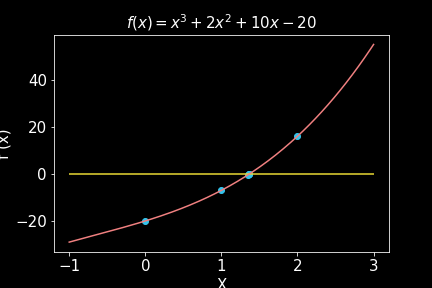
\includegraphics[scale=0.8]{muellergraphic.png}
  \caption{Mueller Algortihm, the blue dots represent the x values chosen for the parabola construction}
  \label{muellergraphic}
\end{figure}


\section{Gaussian Elimination}
For Gaussian Elimination we are allowed 3 types of operations to get to the row reduced form:

\begin{itemize}
 \item Swapping two rows
 \item Multiplying a row by a nonzero number
 \item Adding a multiple of one row to another row
\end{itemize}

So using these three rules, we can solve $AX=B$, where A is defined as
$$A = \begin{bmatrix}
  10 & -7 & 3 & 5\\
  -6 & 8 & -1 & -4 \\
  3&1&4&11 \\
  5&-9&-2&4

\end{bmatrix};
B =
\begin{bmatrix}
6\\
5\\
2\\
7 \end{bmatrix}$$
We start with:
$\begin{vmatrix}
10 & -7 & 3 & 5\\
-6 & 8 & -1 & -4 \\
3&1&4&11 \\
5&-9&-2&4
\end{vmatrix}\begin{matrix}
6\\
5\\
2\\
7 \end{matrix} $ and try to end with something like $\begin{vmatrix}
1 & 0 & 0 & 0\\
0 & 1 & 0 & 0 \\
0&0&1&0 \\
0&0&0&1
\end{vmatrix}\begin{matrix}
h\\
i\\
j\\
k \end{matrix} $ \\ \\ \\
Step 1: $R_1 /10 \rightarrow R_1$
$\begin{vmatrix}
1 & -0.7 & 0.3 & 0.5\\
-6 & 8 & -1 & -4 \\
3&1&4&11 \\
5&-9&-2&4
\end{vmatrix}\begin{matrix}
0.6\\
5\\
2\\
7 \end{matrix} $
\\ \\ \\
Step 2: $R_2 + 6R_1 \rightarrow R_2$; $R_3 - 3R_1 \rightarrow R_3$; $R_4 - 5R_1 \rightarrow R_4$
$\begin{vmatrix}
1 & -0.7 & 0.3 & 0.5\\
0 & 3.8 & 0.8 & -1 \\
0&3.1&3.1&9.5 \\
0&-5.5&-3.5&1.5
\end{vmatrix}\begin{matrix}
0.6\\
8.6\\
0.2\\
4 \end{matrix} $
\\ \\ \\
Step 3: $R_2 / 3.8 \rightarrow R_2$
$\begin{vmatrix}
1 & -0.7 & 0.3 & 0.5\\
0 & 1 & \frac{4}{19} & -\frac{5}{19} \\
0&3.1&3.1&9.5 \\
0&-5.5&-3.5&1.5
\end{vmatrix}\begin{matrix}
0.6\\
\frac{43}{19}\\
0.2\\
4 \end{matrix} $
\\ \\ \\
Step 4: $R_1 + 0.7R_2 \rightarrow R_1$; $R_3 - 3.1 R_2 \rightarrow R_3$; $R_4 + 5.5 R_2 \rightarrow R_4$
$\begin{vmatrix}
1 & 0 & \frac{17}{38} & \frac{6}{19}\\
0 & 1 & \frac{4}{19} & -\frac{5}{19} \\
0&0&\frac{93}{38}&\frac{196}{19} \\
0&0&-\frac{89}{38}&\frac{1}{19}
\end{vmatrix}\begin{matrix}
\frac{83}{38}\\
\frac{43}{19}\\
-\frac{259}{38}\\
\frac{625}{38} \end{matrix} $
\\ \\ \\
Step 5: $R_3 / \frac{93}{38}  \rightarrow R_3$
$\begin{vmatrix}
1 & 0 & \frac{17}{38} & \frac{6}{19}\\
0 & 1 & \frac{4}{19} & -\frac{5}{19} \\
0&0&1&\frac{392}{93} \\
0&0&-\frac{89}{38}&\frac{1}{19}
\end{vmatrix}\begin{matrix}
\frac{83}{38}\\
\frac{43}{19}\\
-\frac{259}{93}\\
\frac{625}{38} \end{matrix} $
\\ \\ \\
Step 6: $R_1 - \frac{17}{38}R_3  \rightarrow R_1$; $R_2 - \frac{4}{19}R_3 \rightarrow R_2$; $R_4 + \frac{89}{38}R_3 \rightarrow R_4$
$\begin{vmatrix}
1 & 0 & 0 & -\frac{146}{93}\\
0 & 1 & 0 & -\frac{107}{93} \\
0&0&1&\frac{392}{93} \\
0&0&0&\frac{923}{93}
\end{vmatrix}\begin{matrix}
\frac{319}{93}\\
\frac{256}{93}\\
-\frac{259}{93}\\
\frac{923}{93} \end{matrix} $
\\ \\ \\
Step 7: $R_4 / \frac{923}{93}  \rightarrow R_4$;
$\begin{vmatrix}
1 & 0 & 0 & -\frac{146}{93}\\
0 & 1 & 0 & -\frac{107}{93} \\
0&0&1&\frac{392}{93} \\
0&0&0&1
\end{vmatrix}\begin{matrix}
\frac{319}{93}\\
\frac{256}{93}\\
-\frac{259}{93}\\
1 \end{matrix} $
\\ \\ \\
Step 8: $R_1 + \frac{146}{93}R_4  \rightarrow R_1$;  $R_2 + \frac{107}{93}R_4 \rightarrow R_2$;  $R_3 = \frac{392}{93}R_4 \rightarrow R_3 $
$\begin{vmatrix}
1 & 0 & 0 &0\\
0 & 1 & 0 & 0 \\
0&0&1&0 \\
0&0&0&1
\end{vmatrix}\begin{matrix}
5\\
4\\
-7\\
1 \end{matrix} $
\\ \\ \\
Thus $X = \begin{bmatrix}
5\\
4\\
-7\\
1 \end{bmatrix}$ and to check we can plug in these values into the equations, which I give the first for example:
$$10(5) - 7(4) + 3(-7) + 5(1) = 6$$ ( hopefully its okay I do not show the rest, but trust me they work out ;) )

\begin{figure}
  \centering
  \includegraphics[scale=0.5]{muellerscode.png}
  \caption{Code can also be found in Link to Github }
  \label{muellercode}
\end{figure}
\end{document}
